\subsection{Python, Sympy, Numpy, Scipy y Matplotlib}

El lenguaje de programación Python está por defecto desprovisto de capacidades de cálculo científico e ingenieril.  Esta es una decisión de diseño para hacer que tales funcionalidades deban ser agregadas por bibliotecas especializadas. El efecto de esta decisión es que el desarrollo de las mismas corre por cuenta de usuarios que las aplican en diversos ámbitos del desarrollo científico-tecnológico antes que por profesionales de las informática.

Las funciones del cálculo simbólico las provee la biblioteca Sympy. Se aprovecha en particular su módulo Mechanics que facilita la generación de ecuaciones para la dinámica de sistemas de cuerpos rígidos con múltiples grados de libertad y en variados sistemas de referencia \cite{simpy}.

Los sistemas de ecuaciones diferenciales se resuelven por métodos numéricos apoyados en las funciones para la manipulación de elementos algebraicos de la biblioteca Numpy \cite{numpy} y de los algoritmos de optimización e integración numérica de Scipy \cite{SciPy}.

El análisis en ingeniería de resultados numéricos son usualmente interpretados con representaciones gráficas. Esta capacidad la proveen las funciones de la biblioteca Matplotilb \cite{matplotlib}.

\subsection{Cuadernos de Jupyter}

El entorno usado en el curso para ejecutar código es la aplicación basada en la web del Proyecto Jupyter llamada JupyterLab cuyo  formato de documento es el cuaderno (notebook) Jupyter \cite{Kluyver2016jupyter}. Este alterna secciones independientes denominadas celdas. Las de entrada son de código (en variados lenguajes, Python es solo uno de los posibles) o de  anotaciones, como muestra la figura \ref{fig:jupyter}. Esta última variante de celdas se escriben en el lenguaje de  marcado Markdown \cite{markdown} que permite incrustar: texto y/o expresiones matemáticas en formato \LaTeX intercaladas, y contenido multimedia: enlaces web, imágenes, reproductores de video o sonido.

\begin{figure}[!ht]
\centering
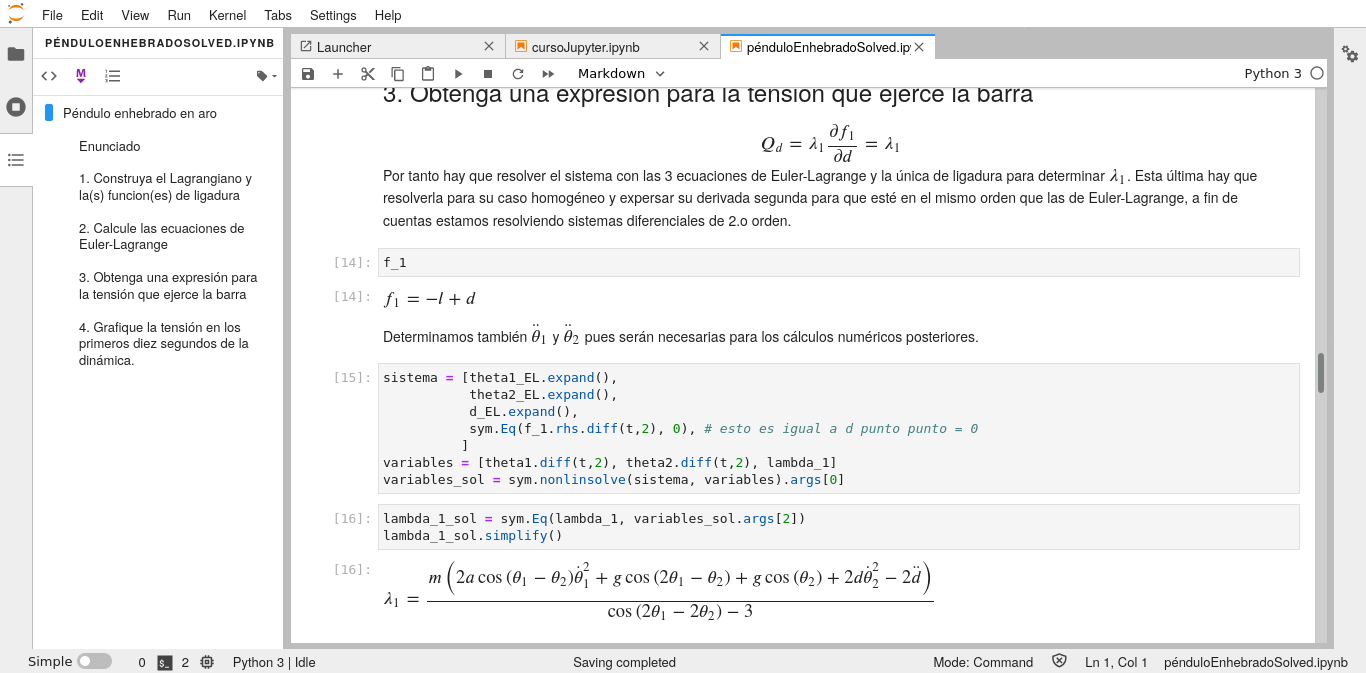
\includegraphics[width=3.5in]{figuras/screenshot_JupyterLab.png}
\caption{Un cuaderno de Jupyter es un conjunto de celdas. Estas son en formato Markdown o de código ejecutable. Las primeras pueden contener texto,  expresiones  matemáticas o contenido multimedia. Las segundas líneas de código en variados lenguajes de programación. Intercalando títulos en las celdas Markdown se genera el índice (a la izquierda) que facilita la ubicación dentro del documento.}
\label{fig:jupyter}
\end{figure}

La utilización de sintaxis \LaTeX para la simbología matemática provee una notación clara estandarizada bajo los lineamientos de la American Mathematical Society \cite{ams}.
El resultado de la ejecución de una celda de código muestra al usuario el resultado que el mismo instruye a la computadora imprimir. En el curso estas últimas incluyen tanto los comandos para realizar cálculos así como la resolución de un sistema de ecuaciones no lineales que se imprime en la última celda del cuaderno mostrado en la figura 2.  

\subsection{Ejecución de Jupyter en línea}

No se impone a los estudiantes el instalar ningún software para cursar la materia en su dispositivo informático. Solo requieren utilizar un navegador web estándar para utilizar alguno de los servicios que ejecutan cuadernos de Jupyter en línea. Este puede tratarse de una instalación de JupyterHub del Proyecto Jupyter en servidores propios de la universidad o en nubes comerciales, o en su defecto de alguno de los servicios que ofrecen alternativas incluso gratuitas como, entre otras, CoCalc, IBM Watson o Google Colaboratory. De estas se ha utilizado esta última en las últimas ediciones del curso tras cerrar Microsoft su servicio gratuito Azure Notebooks.

El servicio Google Colaboratory, coloquialmente sólo Colab,  presenta como conveniencia el poder ejecutar cuadernos alojados en un repositorio Git gerenciado por el servicio en línea GitHub. Basta una modificación en el URL de un cuaderno para que este apunte a un navegador web a ejecutarle en Colab \cite{colab}. El trabajo con cuadernos Jupyter en este servicio puede realizarse en forma concurrente por parte de varios alumnos y/o docentes. También pueden incluirse comentarios cuya actualización es reportada por correo electrónico lo que es útil para la corrección de los ejercicios pues pueden indicarse la ubicación de errores en el código como muestra la figura \ref{fig:colab}.

\begin{figure}[!ht]
\centering
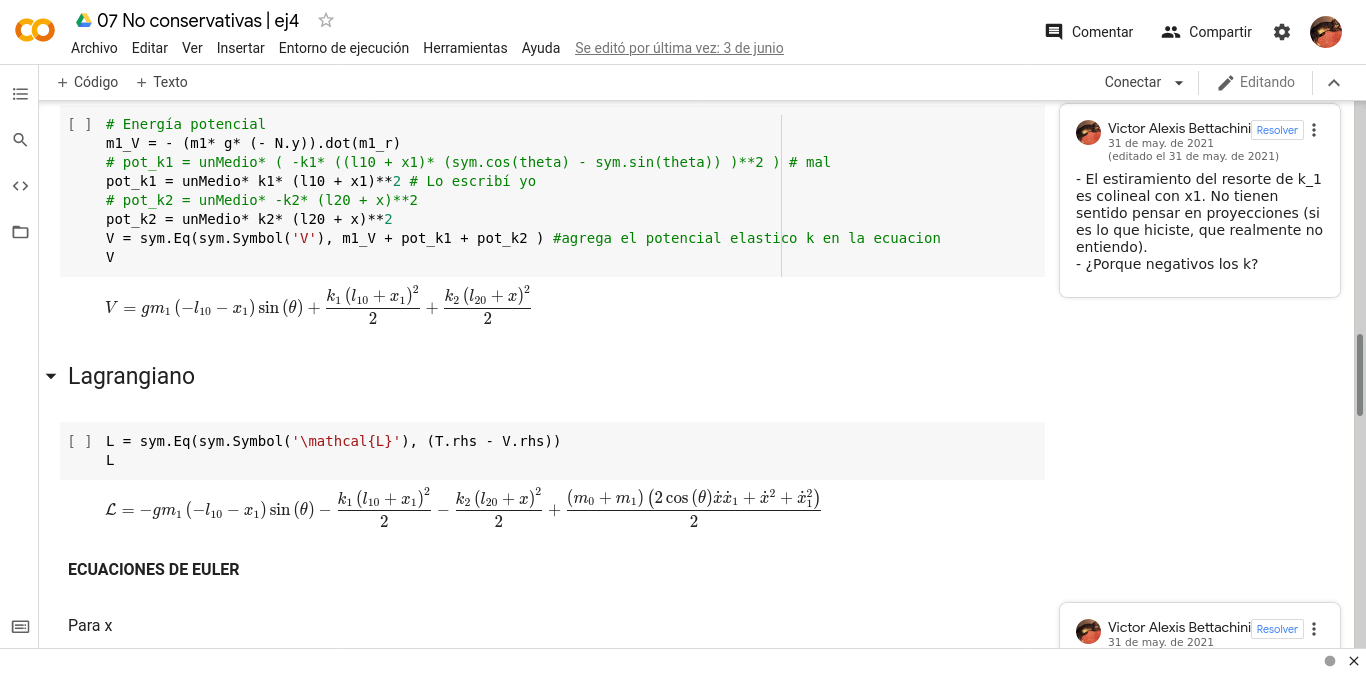
\includegraphics[width=3.5in]{figuras/comentariosColab.png}
\caption{El sitio web Google Colaboratoy permite editar y ejecutar cuadernos Jupyter en forma concurrente entre alumnos y docentes además de incluir comentarios. Esta última característica es útil para las correcciones.}
\label{fig:colab}
\end{figure}

\subsection{Repositorio Git}

El mencionado repositorio en GitHub está organizado en sendas carpetas por clase del curso, como muestra la figura \ref{fig:github}. Cada una de estas aloja el correspondiente material teórico y ejercicios en el formato de cuadernos Jupyter además de  guías de ejercicios y algún apunte ocasional en el formato de documento portátil conocido por su sigla en inglés PDF. Este ordenamiento facilita tanto al docente como a los alumnos una vista de conjunto del material de cada temática así como el verificar las eventuales actualizaciones del mismo. De esta forma el material del curso es de acceso público haciéndolo disponible para ser utilizado a interesados \cite{repositorio-victor} mientras cumplan con citar su origen y no darle uso comercial como indica su licencia Creative Commons CC-BY-NC-SA bajo el que está publicado \cite{creative}.

\begin{figure}[!ht]
\centering
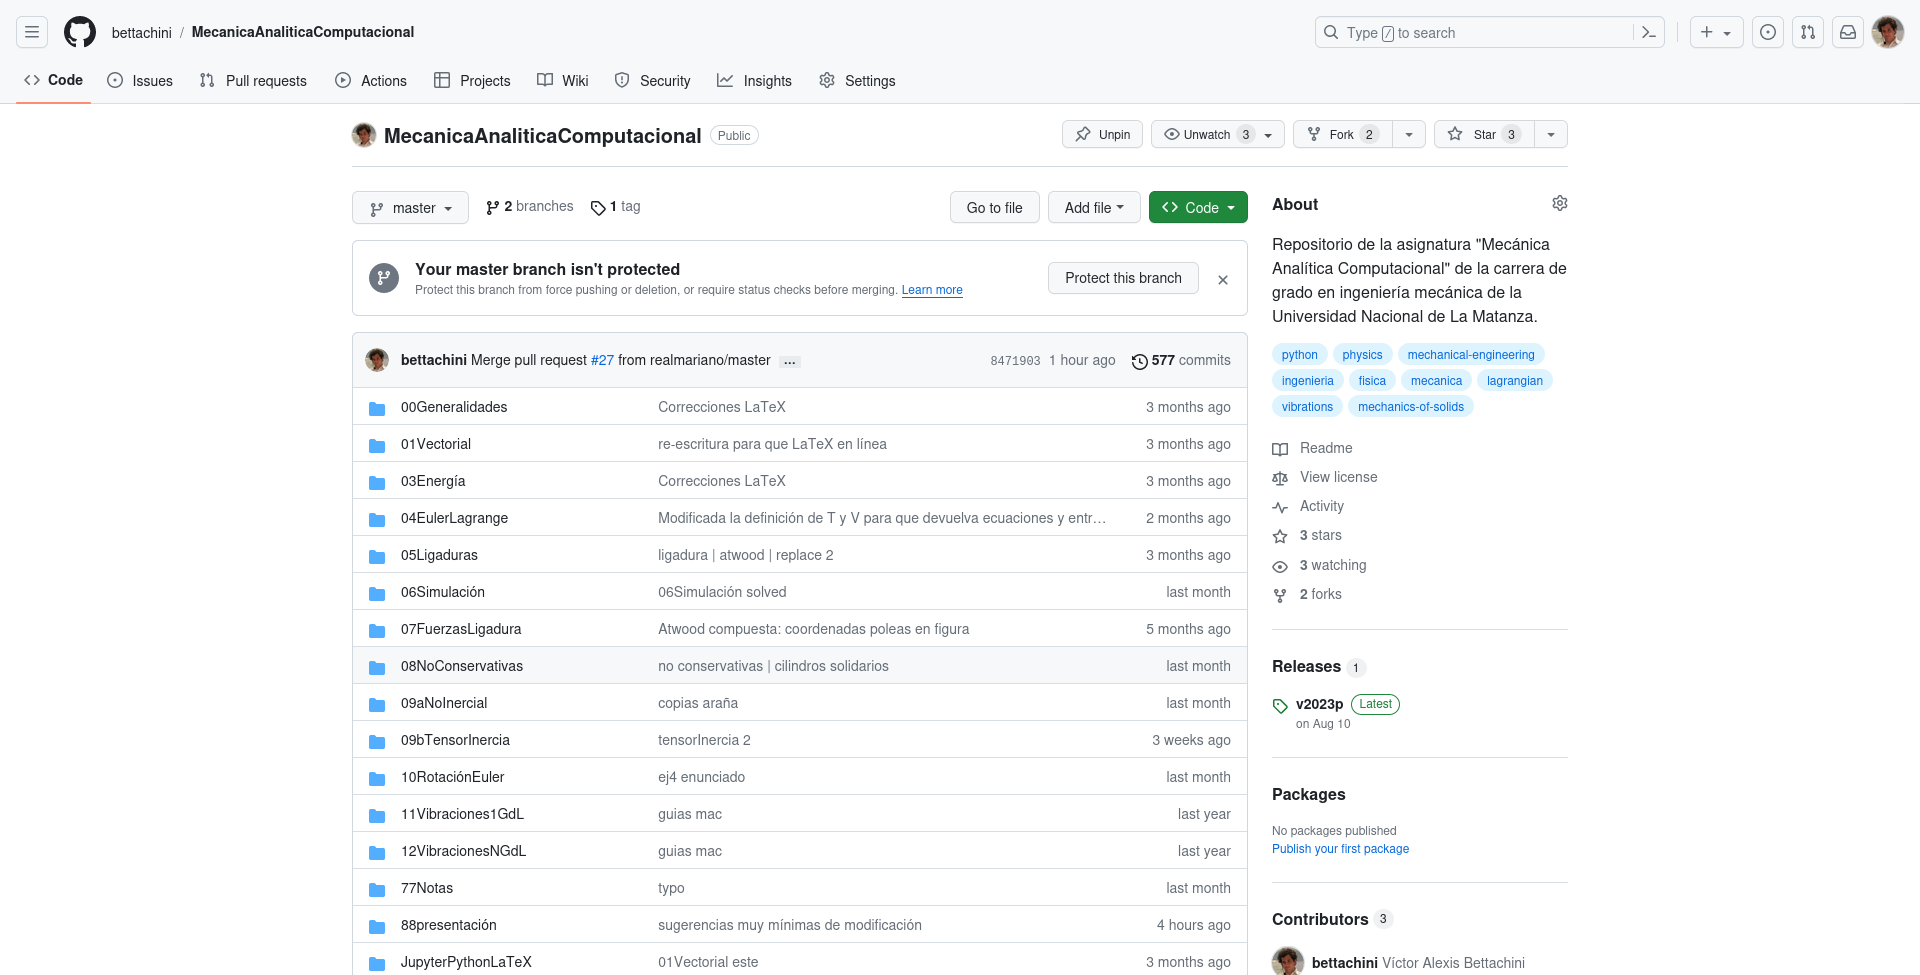
\includegraphics[width=3.5in]{figuras/repositorioGithub.png}
\caption{Los alumnos encuentran el material ordenado en sendos directorios por clase.}
\label{fig:github}
\end{figure}

\subsection{Sistema de gestión de aprendizaje}

En la UNLaM se utiliza la plataforma de comunicaciones de negocios Microsoft Teams para suplir la interacción en el aula con los alumnos con videoconferencias. Luego de terminada cada clase el video de las mismas se guarda en el almacenamiento en línea Microsoft OneDrive. Enlaces a estos y a los materiales de la clase alojados en el repositorio Git se  compartimentan en lo que el sistema llama canales respetando la misma numeración y denominación que en el repositorio Git. La figura \ref{fig:teams} muestra los contenidos que encabezan los desplegados para la décima clase.

En cada canal se incluyen enlaces a:
\begin{itemize}
    \item guía de ejercicios prácticos
    \item algún eventual apunte en PDF
    \item ambas vías para ver los cuadernos Jupyter, la interactiva en Colab o estática en nbviewer
    \item invitación a la videoconferencia o a su video una vez esta terminó
\end{itemize}

Microsoft Teams provee también los rudimentos de un sistema de gestión de aprendizaje (LMS por sus siglas en inglés) al permitir asignar tareas a alumnos con fechas límites de aceptación por parte del sistema. Los alumnos pueden cargar al sistema un enlace a su cuaderno en Colab o el mismo en formato .ipynb en el caso de que no se permita modificación del mismo con posterioridad a una fecha por cuestiones de evaluación.

\begin{figure}[!ht]
\centering
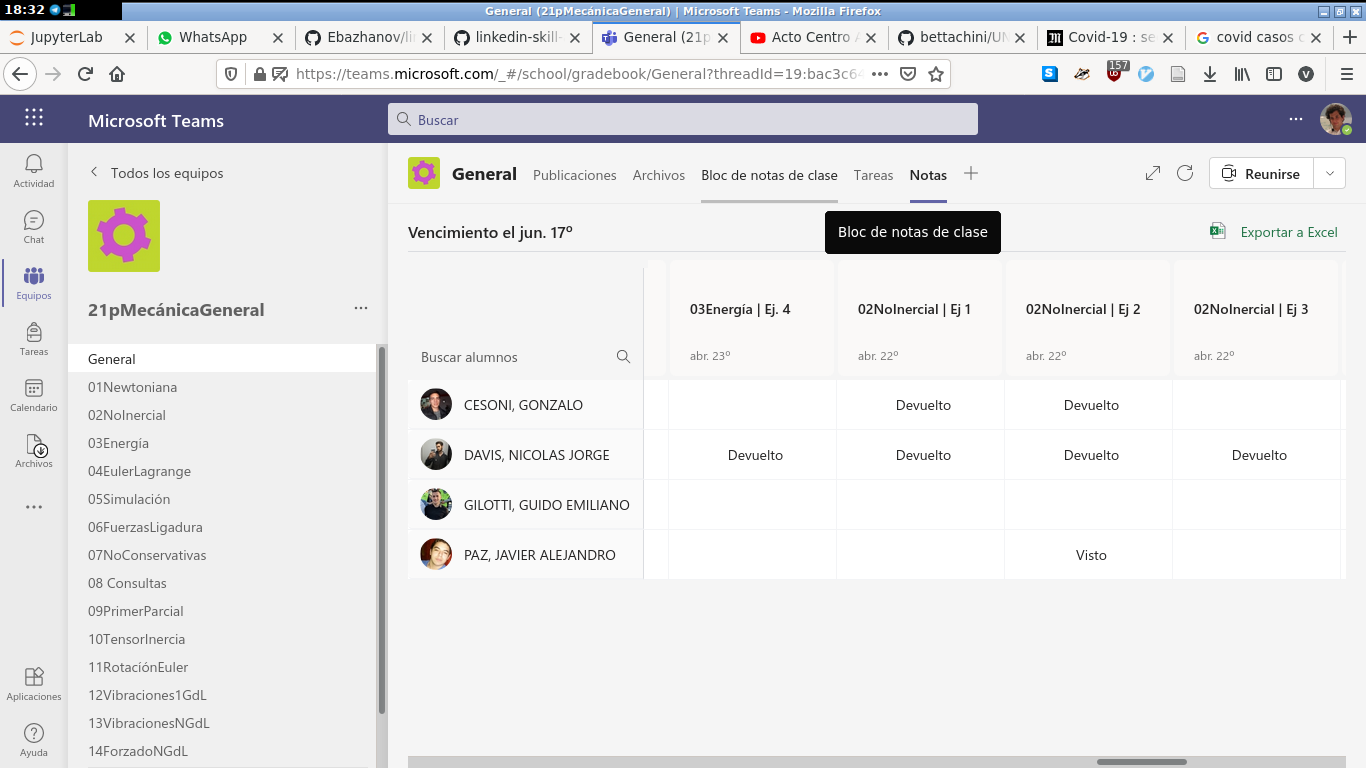
\includegraphics[width=3.5in]{figuras/notasTeams.png}
\caption{Sendos canales por clase presentan los enlaces a su material.}
\label{fig:teams}
\end{figure}